\chapter{Architektur}
\label{cha:architektur}
In diesem Kapitel werden die architektonischen Randbedingungen für die Entwicklung der Applikation beschrieben. Hierzu zählt welche Anwendungsfälle in den späteren Prototypen und im schlussendlichen Messeprototyp gegeben sein muss. Daraus resultiert der Aufbau der Datenbank und die schlussendliche Systemarchitektur. Als Grundlage dient das Pflichtenheft. Dieses liegt dieser Arbeit gesondert im Anhang bei (siehe Anhang \ref{sec:Pflichtenheft}).

\section{Anwendungsfälle}
\label{sec:anwendungsfaelle}
Das Pflichtenheft sieht eine Unterteilung des Projekts in zwei aufeinanderfolgenden Meilensteine vor. Hierbei werden erst Proof-of-Concept-Prototypen entwickelt. Anschließend wird ein Prototyp zum Messe-Prototypen weiterentwickelt. \\
Für diese beiden Prototypen müssen andere bzw. erweiterte Anwendungsfälle implementiert werden. Darum werden nachfolgend für die beiden Implementierungsschritte die Anwendungsfälle einzeln aufgeschlüsselt. 
\subsection{Anwendungsfälle für Meilenstein 1 (Proof-of-Concept-Phase)}
\label{ssec:anwendungsfaelle-poc}
Aus dem Pflichtenheft ergeben sich folgende Anwendungsfälle für die erste Phase des Projekts:
\begin{itemize}
\item Es soll möglich sein, sich an der Anwendung anzumelden
\item Es soll möglich sein, eine Entität mit Daten (Trainingsplan, Training oder Übung) unabhängig von der Verbindung zum Web Service persistent anzulegen, zu ändern und zu speichern
\item Optional soll sich ein Nutzer an der Anwendung registrieren können
\end{itemize}

\begin{figure}[h]
\centering
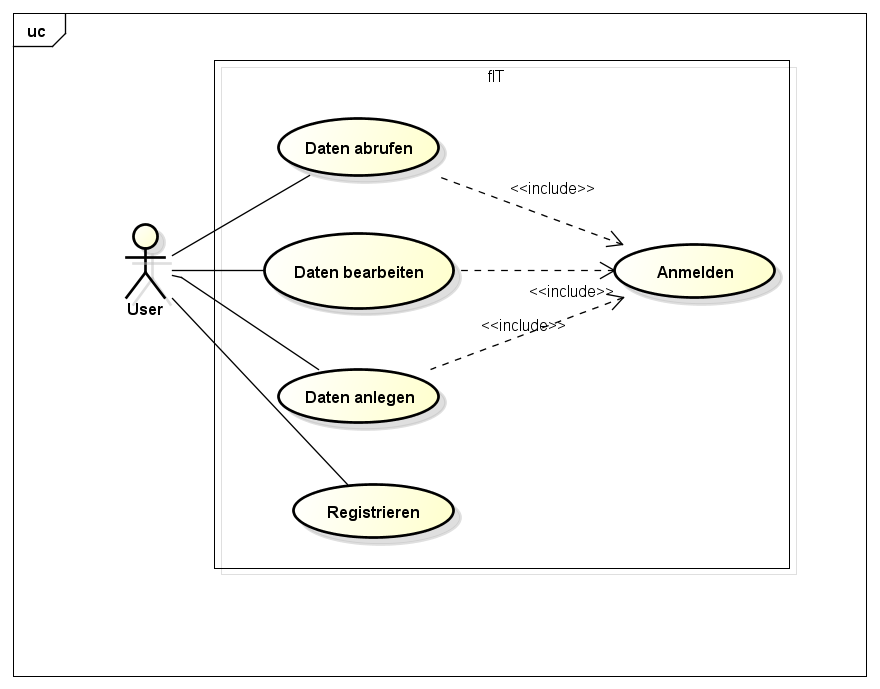
\includegraphics[width=0.8\linewidth]{content/images/UseCase-Proof-of-Concept.png}
\caption{Use-Cases Proof-of-Concept}
\label{pic:usecase-poc}
\end{figure}

\subsection{Anwendungsfälle für Meilenstein 2 (Messe-Prototyp-Phase)}
\label{ssec:anwendungsfaelle-messe}
Für den Meilenstein 2 werden die bereits vorgestellten Anwendungsfälle weiter verfeinert. Daraus ergeben sich folgende Anwendungsfälle:
\begin{itemize}
\item Ein Nutzer soll sich an der Anwendung anmelden können.
\item Ein Nutzer soll seine eigenen Trainingsplan-Daten abrufen können
\item Ein Nutzer soll zu einem seiner Trainingspläne alle zugehörigen Übungen abrufen können
\item Ein Nutzer soll zu einer dieser Übungen seine bisherigen Trainingsdaten abrufen können
\item Ein Nutzer soll zu einer Übung ein neues Training anlegen können
\item Alle nicht-optionalen Anwendungsfälle müssen unabhängig von einer Serververbindung funktionieren und eventuell anfallende Daten dauerhaft speichern.
\item Optional: Ein Nutzer soll eine Statistik der letzten Trainings zu einer Übung abrufen können. Neu erstellte Trainingsdaten aktualisieren diese Statistik
\item Optional: Ein Nutzer soll sich an der Applikation registrieren können
\item Optional: Ein Nutzer mit der Rolle \textit{Administrator} soll neue Übungen anlegen können
\end{itemize}

\begin{figure}[h]
\centering
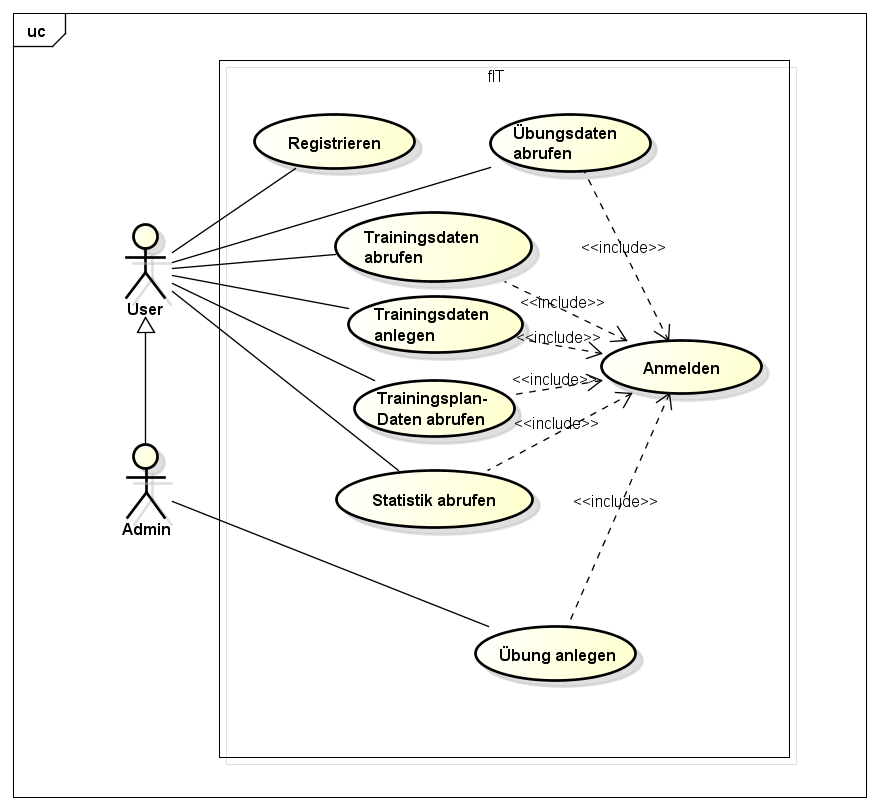
\includegraphics[width=0.8\linewidth]{content/images/UseCase-Messeprototyp.png}
\caption{Use-Cases Messeprototyp}
\label{pic:usecase-messe}
\end{figure}
\newpage
\section{Datenbank-Entwurf}
\label{sec:Datenbank-Entwurf}
Aus den definierten Anwendungsfälle ergibt sich die Struktur für die Datenbank. Als Grundlage werden die Anwendungsfälle des zweiten Meilensteins genutzt, um spätere Anpassungen nach Beendigung des ersten Meilensteins zu vermeiden.

\begin{figure}[h]
\centering
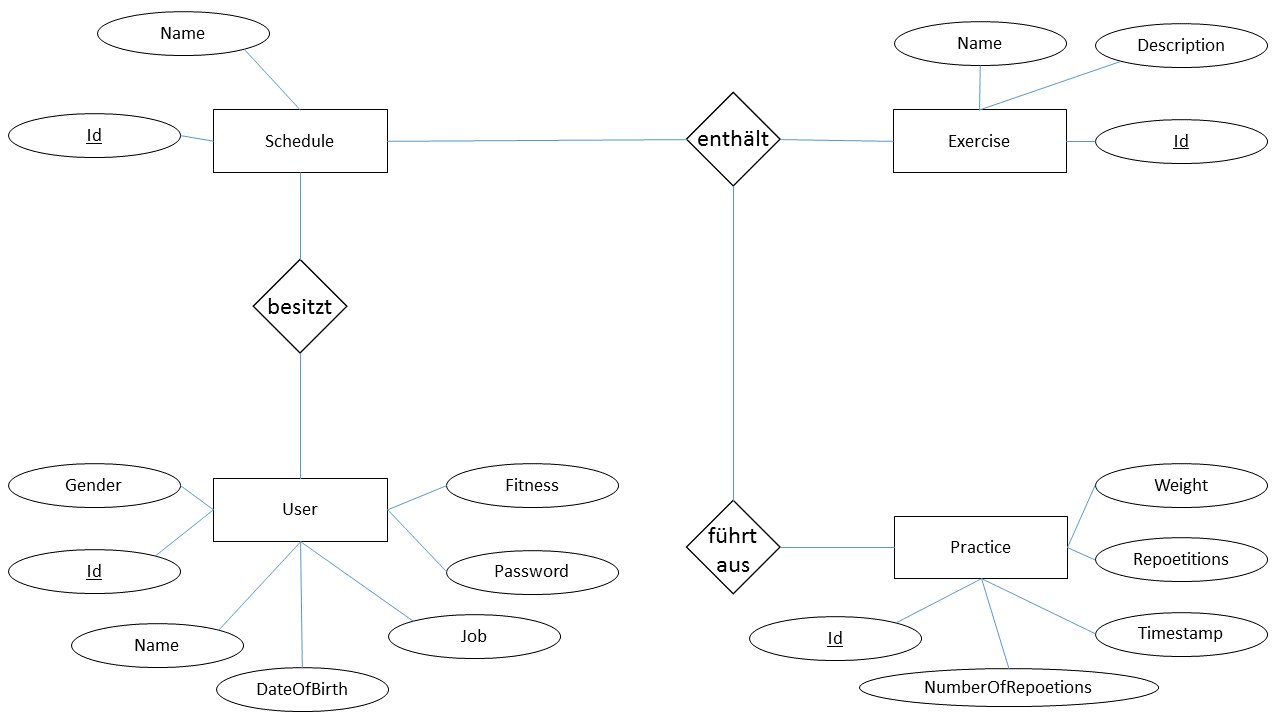
\includegraphics[width=0.8\linewidth]{content/images/DB-Entwurf.png}
\caption{Datenbank-Entwurf}
\label{pic:usecase-messe}
\end{figure}

\section{Programmarchitektur}
\label{sec:programmarchitektur}
Da verschiedene Clients implementiert werden sollen, ist es sinnvoll das Projekt als Mehrschichtenarchitektur für verteilte Anwendung zu implementieren. \\
Der Server hält dabei die Funktionen zur Nutzung durch die Clients vor. Konkret greift der Server per OR-Mapper auf die Datenbank zu, bereitet die Daten in der Applikations-Schicht auf und reicht sie über eine Rest-Schnittstelle an die anfragenden Client weiter. Dabei muss gewährleistet sein, dass ein Nutzer nur die Daten abrufen darf, für die er autorisiert wurde. \\
Clientseitig werden Daten in einer Caching-Schicht zum Schutz vor eventuellen Verbindungsabbrüchen zwischengespeichert. Anschließend werden die erhaltenen Daten auf dem Endgerät für die Anzeige aufbereitet und angezeigt. \\
Abbildung \ref{pic:architecture} bildet diesen Aufbau grafisch ab:
\begin{figure}[h]
\centering
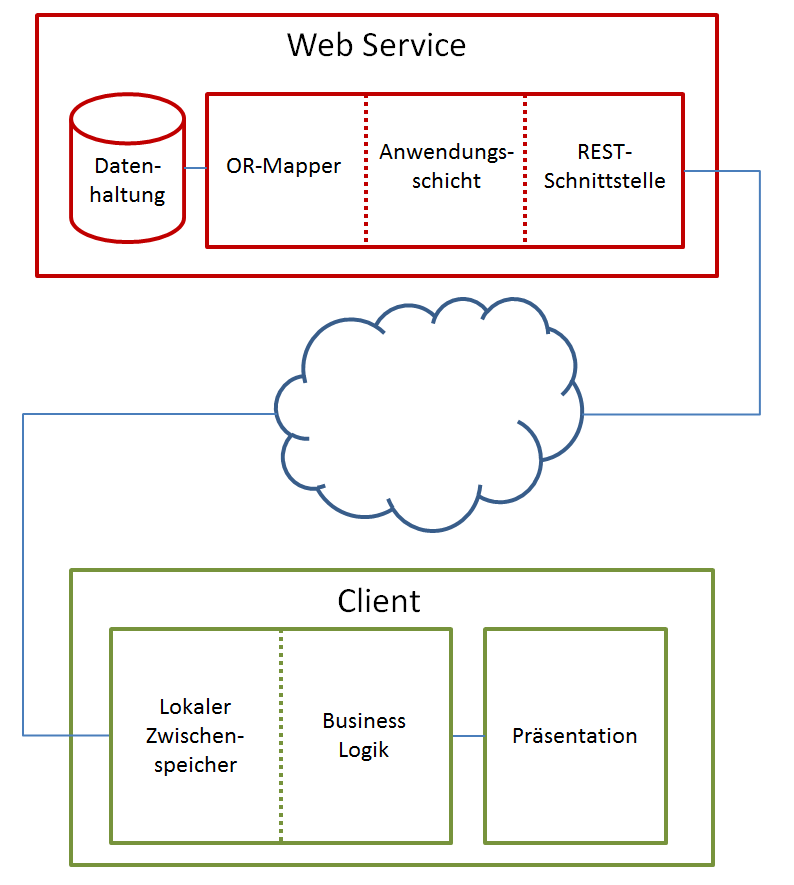
\includegraphics[width=0.8\linewidth]{content/images/Aufbau-Architektur.png}
\caption{Aufbau der Anwendung}
\label{pic:architecture}
\end{figure}
\section{Rollen-Konzept}
\label{sec:rollen-konzept}
Im Pflichtenheft wird für den zweiten Meilenstein eine Unterscheidung in den Berechtigungen gemacht (Nur Administrationen dürfen neue Übungen anlegen). Darum ist es nötig, ein Rollenkonzept zu entwickeln, der den Zugriff auf bestimmte Ressourcen reguliert. \\
Aus den Aussagen, die im Pflichtenheft getroffen wurden, geht hervor, dass sich der Nutzer in mindestens einem der folgenden Zustände befindet:
\begin{itemize}
\item unautorisiert
\item Rolle \textit{Nutzer}
\item Rolle \textit{Administrator}
\end{itemize}